\documentclass[a4paper,11pt]{article}
\pdfoutput=1 % if your are submitting a pdflatex (i.e. if you have
             % images in pdf, png or jpg format)
\usepackage{amsmath}
\usepackage{jheppub} % for details on the use of the package, please
                     % see the JHEP-author-manual
\usepackage{multicol}
\usepackage{scrextend}
\usepackage[dvipsnames]{xcolor}
\usepackage{tikz}
\usepackage[T1]{fontenc} % if needed

\newcommand{\bP}{\mathbb{P}}
\newcommand{\bZ}{\mathbb{Z}}
\newcommand{\bC}{\mathbb{C}}
\newcommand{\bE}{\mathbb{E}}
\newcommand{\bR}{\mathbb{R}}
\newcommand{\cO}{\mathcal{O}}
\newcommand{\cT}{\mathcal{T}}
\newcommand{\cS}{\mathcal{S}}
\newcommand{\cA}{\mathcal{A}}
\newcommand{\cN}{\mathcal{N}}
\newcommand{\cD}{\mathcal{D}}
\newcommand{\cR}{\mathcal{R}}
\newcommand{\ns}{$n$'s }
\newcommand{\ms}{$m$'s }
\newcommand{\grad}{\nabla}
\newcommand{\jh}[1]{{\color{blue}  #1}}

\newcommand{\tv}{{\tilde v}}

\newcommand{\tV}{{\tilde V}}
\newcommand{\XXX}[3]{{\color{blue}{\bf [#1: } {\tt #3} {\it -#2-}{\bf ]}}}

\newcommand{\hoo}{h^{11}}
\newcommand{\hoomin}{h^{11}_{\text{min}}}
\newcommand{\hoomax}{h^{11}_{\text{max}}}
\newcommand{\sdoc}{S_{\Delta_1^\circ}}
\newcommand{\sdtc}{S_{\Delta_2^\circ}}
\newcommand{\sdc}{S_{\Delta^\circ}}
\newcommand{\dc}{{\Delta^\circ}}
\newcommand{\doc}{{\Delta_1^\circ}}
\newcommand{\dtc}{{\Delta_2^\circ}}



\def\ge{E}
\def\gso{SO}
\def\gsu{SU}
\def\gsp{Sp}
\def\gf{F}
\def\gg{G}

\title{\boldmath Small Cosmological Constants}

% more complex case: 4 authors, 3 institutions, 2 footnotes
%\author[a]{Jonathan Carifio,}
%\author[b]{Tina Eliassi-Rad,}
\author[a]{James Halverson,}
\author[a]{Cody Long,}
\author[a]{Brent Nelson,}
\author[b]{Fabian Ruehle}

% The "\note" macro will give a warning: "Ignoring empty anchor..."
% you can safely ignore it.

\affiliation[a]{Department of Physics, Northeastern University,\\Boston, MA 02115, USA}
\affiliation[b]{Rudolf Peierls Centre for Theoretical Physics, Oxford University,\\
1 Keble Road, Oxford, OX1 3NP, UK}

% e-mail addresses: one for each author, in the same order as the authors
% \emailAdd{first@one.univ}
% \emailAdd{second@asas.edu}
% \emailAdd{third@one.univ}
% \emailAdd{fourth@one.univ}




\abstract{

  \vspace{.2cm}
  Note: this being in JHEP format is just for convenience, not saying this is necessarily for JHEP.

}
  
  

\begin{document} 
\maketitle
\flushbottom

\section{Introduction}

\section{Bousso-Polchinski Problem Setup}



\subsection{The Bousso-Polchinski Model}

\begin{equation}
\Lambda = \Lambda_0 + g_{ij} N_i N_j
\end{equation}

\begin{equation}
Vol(L) = \frac{\left(\pi L\right)^{k/2}}{(k/2)! \, \sqrt{det g}}
\end{equation}

\begin{equation}
\delta Vol = \frac{k}{2\Lambda_0} \, Vol(|\Lambda_0|) \, \epsilon
\end{equation}

For simplicity we set $M_\text{pl}=1$ and then $\Lambda_0 = -1$.
Having many vacua with cosmological constants in the BP shell, and also
having the volume approximate the number of lattice points in the shell,
requires $\delta Vol >> 1$. We will henceforth refer to this as shell volume
condition (SVC). In this language, one critical observation of Bousso-Polchinski
is that at large $k$ the SVC condition is automatically satisfied
and there are an exponentially large number of vacua with
small cosmological constant.

However, our applications will begin for simplicity at small
$k$, and therefore we must analyze conditions under which
the SVC condition is satisfied. Specifically, for any
fixed value of $k$ we would like to know regimes in which
$det \, g$ and $\epsilon$ are such that they allow for an
exponentially large number of vacua with cosmological
constant of order $\epsilon$. To do this it is useful
to express the problem in terms of a parameter
that has
mass dimension one, $\mu$ such that $\mu^4:=(det\, g)^{1/k}$,
where $g$ has mass dimension $[g]=4$ because in our
convention the flux vectors $N_i$ are dimensionless.
This yields
\begin{equation}
Vol(k,\mu) = \frac{\pi^{k/2}}{\mu^{2k}(k/2)!}, \qquad \delta Vol(k,\mu) = \frac{k Vol(k,\mu)}{2} \, \epsilon,
\end{equation}
and contours for $log_{10}(\delta Vol(k,\mu,\epsilon))$ are presented
in Figure \ref{fig:dvols}. There we see, at large $k$, the 
observation of BP that the number of vacua is exponentially
large for many values of $\mu$ and $\epsilon$.
At small $k$ such as $k=5,10$, we see a $\delta Vol = 1$ contour
that cuts across the plot, signifying the absence of vacua
with $O(\epsilon)$ cosmological constant above that contour.
This means that at small fixed $(k,\epsilon)$ 
we must evaluate whether it is reasonable in a possible metric 
ansatz to actually obtain solutions to the problem; we will find
that is is the case, and choose physically reasonable parameters
for the metric ansatz accordingly.

\begin{figure}
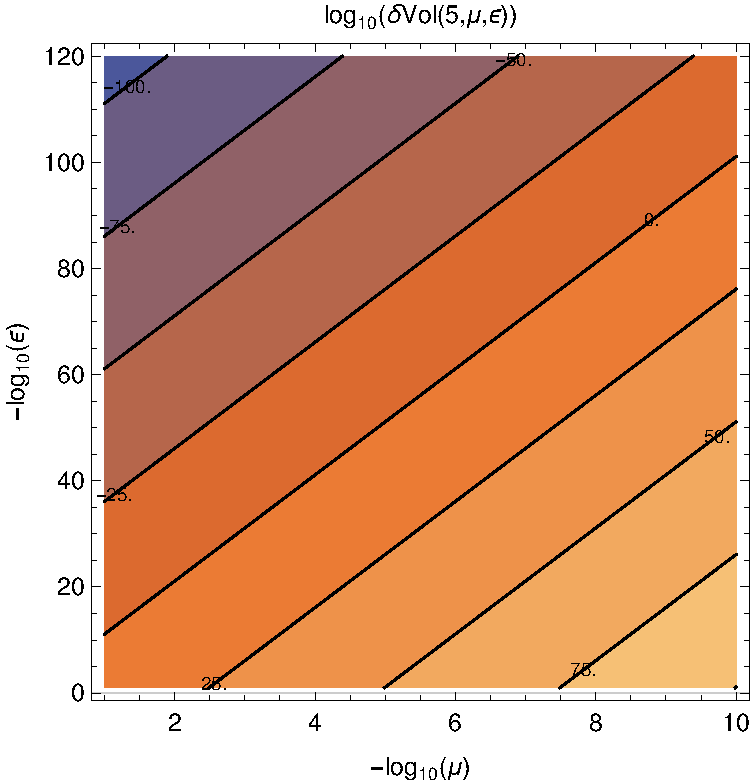
\includegraphics[scale=.6]{dvolk5}
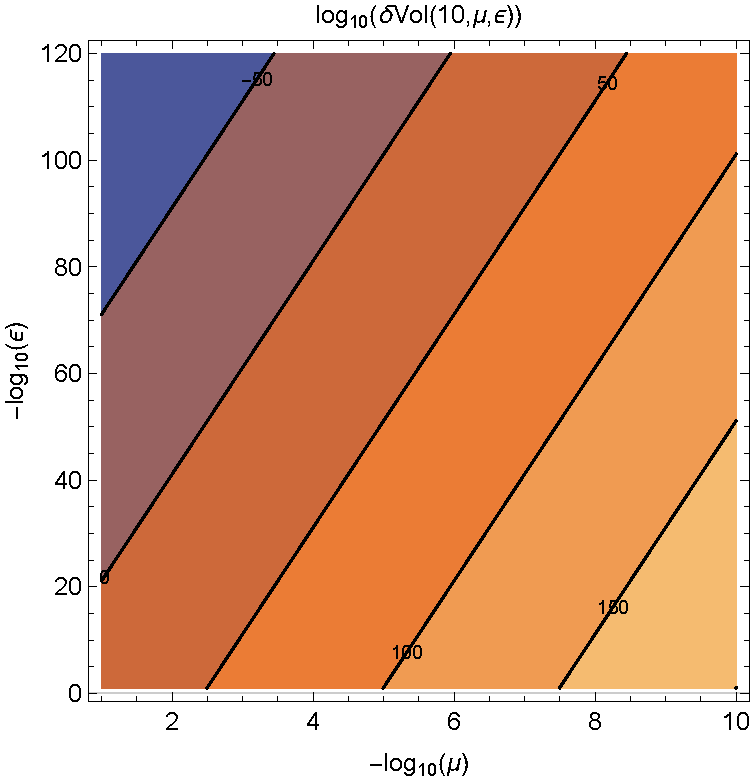
\includegraphics[scale=.6]{dvolk10} \\
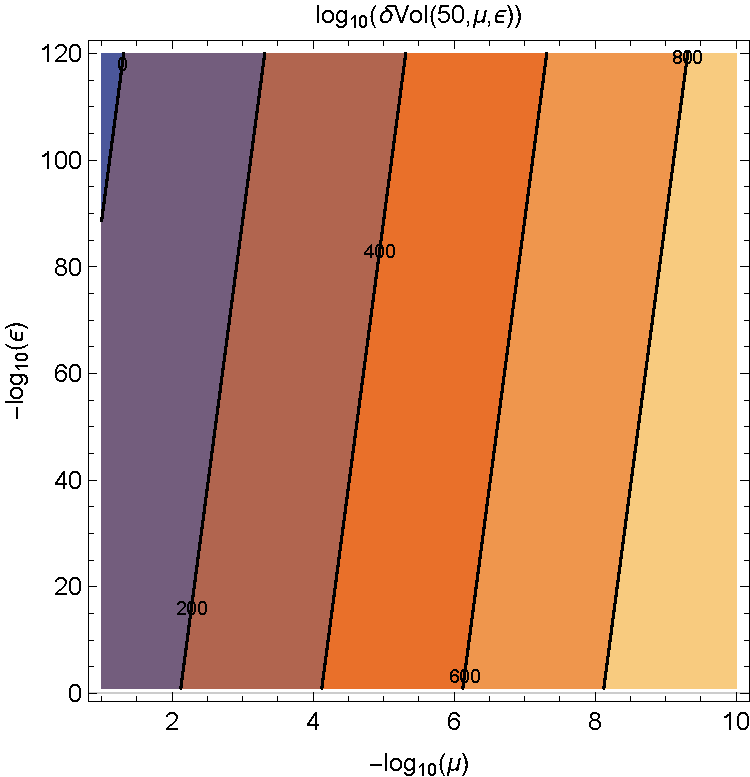
\includegraphics[scale=.6]{dvolk50}
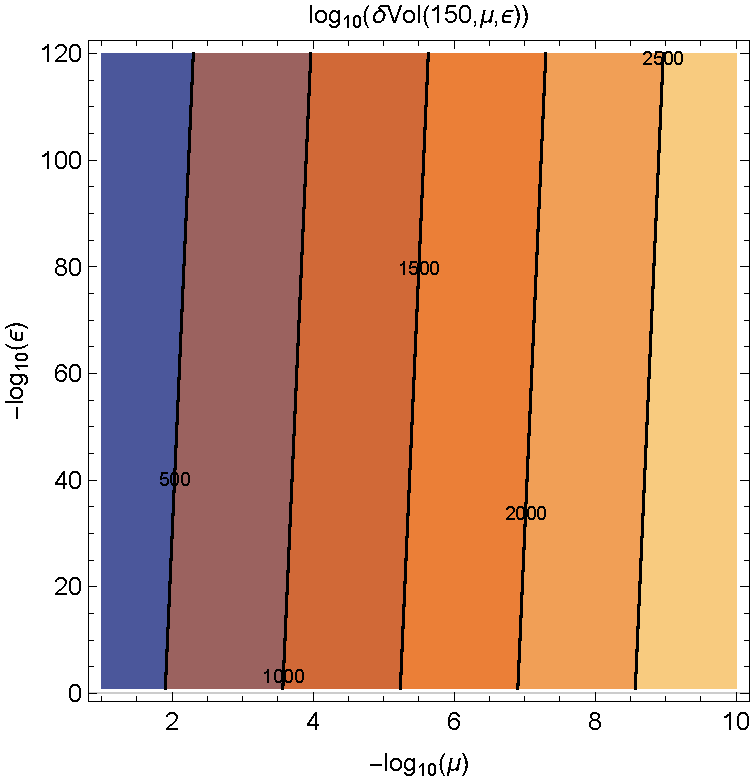
\includegraphics[scale=.6]{dvolk150} 
\caption{Shell volumes for $k=(5,10,50,150)$ as a function of $(\mu,\epsilon)$, beginning with the upper left and moving to the bottom right. \jh{Do you guys know
a way to use the same gradient colors across all plots? Only relevant if
these make the paper.}}
\label{fig:dvols}
\end{figure}


\subsection{Bousso-Polchinski with Wishart Metrics}
Any positive definite $k\times k$ metric $g$ may be written as
\begin{equation}
g = A^\dagger A
\end{equation}
where $A$ is a $Q\times k$ matrix. We choose $g$ to be from the
Wishart distribution by requiring that $A$ is real with entries drawn from a Gaussian distribution with standard deviation $\sigma$. Throughout, we
will choose $Q=k$ for simplicity.

We would like to ask how the requirement of many vacua via the SVC
may be satisfied in the Wishart distribution. There the dependence of the
general shell volume on the triple $(k,\epsilon,det g)$ may be recast into
a dependence on $(k,\epsilon,\sigma)$. This may be done by using the
fact that
\begin{equation}
E[log\, det \, g] = \Psi_k(k/2) + k \,ln(2) + 2 k \,ln(\sigma),
\end{equation}
and therefore $E[det \, g]\propto \sigma^{2k}$ and $
E[\delta Vol] \propto \sigma^{-k}$.  This scaling of $E[det \, g]$ with
$\sigma$ is easily verified in simple numerical experiments. 
\jh{ten line code commented out in tex file}
% import numpy as np
% def random_metric(sigma,nmod): # pos def metric
%     A = np.random.normal(size=(nmod,nmod), scale = sigma)
%     return np.dot(A,A.transpose())
% metdetssig = [[]]
% k = 10
% print 'k',k
% for sig in range(1,10):
%     metdets = [np.linalg.det(random_metric(sig*1e-5,k)) for p in range(100000)]
%     metdetssig.append(metdets)
% for i in range(2,10):
%     print np.mean(metdetssig[i-1])/np.mean(metdetssig[i]), (1.0*(i-1)/i)**(2*k)
$\Psi_k(z)$ is the multivariate digamma function,
\begin{equation}
\sum_{i=1}^k \Psi\left(z+\frac{1-i}{2}\right),
\end{equation}
where $\Psi(z)$ is the digamma \jh{polygamma? check all this again}
function.


In sampling Wishart metrics, $\sigma$ must be chosen to be sufficiently
small for fixed $\epsilon$, $k$ so that the SVC is satisfies.
Defining $\sigma_t$ to be the threshold value of $\sigma$ for which 
$E[\delta Vol]=1$,
a short calculation then gives
\begin{equation}
\sigma_t = exp\left[\frac{2 ln\left(\frac{k \pi^{k/2} \epsilon}{2 (k/2)!}\right)-\Psi_k(k/2)-k\, ln(2)}{2k}\right],
\end{equation}
and satisfying the SVC requires that $\sigma << \sigma_t$. However,
it is not immediately clear how much smaller $\sigma$ must be.

Instead, we may choose $\sigma$ for fixed $(k,\epsilon)$ such that
there are an exponentially large number of vacua with $O(\epsilon)$
cosmological constants. We may do this by comparing to figure \ref{fig:dvols}
and determining $\sigma$ from $\mu$. A short calculation gives $\sigma = \mu^2 F(k)$ where
\begin{equation}
F(k)=\sqrt{\frac12 e^{-\Psi_k(k/2)/k}}.
\end{equation}
However, since $F(5)=1.1$ and  $F(500)=.10$, the functional
dependence on $k$ is mild enough that $\sigma \sim \mu^2$ 
is a good approximation in the regime $k\in (5,100)$ that
we are interested in.




\section{Small Cosmological Constants}
\subsection{Reinforcement Learning}
\subsection{Genetic Algorithms}
\subsection{Control Experiments}

\section{Discussion}

\bibliographystyle{JHEP}
\bibliography{refs}

\end{document}

%%% Local Variables:
%%% mode: latex
%%% TeX-master: t
%%% End:
